\documentclass[twoside]{book}

% Packages required by doxygen
\usepackage{fixltx2e}
\usepackage{calc}
\usepackage{doxygen}
\usepackage[export]{adjustbox} % also loads graphicx
\usepackage{graphicx}
\usepackage[utf8]{inputenc}
\usepackage{makeidx}
\usepackage{multicol}
\usepackage{multirow}
\PassOptionsToPackage{warn}{textcomp}
\usepackage{textcomp}
\usepackage[nointegrals]{wasysym}
\usepackage[table]{xcolor}

% Font selection
\usepackage[T1]{fontenc}
\usepackage[scaled=.90]{helvet}
\usepackage{courier}
\usepackage{amssymb}
\usepackage{sectsty}
\renewcommand{\familydefault}{\sfdefault}
\allsectionsfont{%
  \fontseries{bc}\selectfont%
  \color{darkgray}%
}
\renewcommand{\DoxyLabelFont}{%
  \fontseries{bc}\selectfont%
  \color{darkgray}%
}
\newcommand{\+}{\discretionary{\mbox{\scriptsize$\hookleftarrow$}}{}{}}

% Page & text layout
\usepackage{geometry}
\geometry{%
  a4paper,%
  top=2.5cm,%
  bottom=2.5cm,%
  left=2.5cm,%
  right=2.5cm%
}
\tolerance=750
\hfuzz=15pt
\hbadness=750
\setlength{\emergencystretch}{15pt}
\setlength{\parindent}{0cm}
\setlength{\parskip}{3ex plus 2ex minus 2ex}
\makeatletter
\renewcommand{\paragraph}{%
  \@startsection{paragraph}{4}{0ex}{-1.0ex}{1.0ex}{%
    \normalfont\normalsize\bfseries\SS@parafont%
  }%
}
\renewcommand{\subparagraph}{%
  \@startsection{subparagraph}{5}{0ex}{-1.0ex}{1.0ex}{%
    \normalfont\normalsize\bfseries\SS@subparafont%
  }%
}
\makeatother

% Headers & footers
\usepackage{fancyhdr}
\pagestyle{fancyplain}
\fancyhead[LE]{\fancyplain{}{\bfseries\thepage}}
\fancyhead[CE]{\fancyplain{}{}}
\fancyhead[RE]{\fancyplain{}{\bfseries\leftmark}}
\fancyhead[LO]{\fancyplain{}{\bfseries\rightmark}}
\fancyhead[CO]{\fancyplain{}{}}
\fancyhead[RO]{\fancyplain{}{\bfseries\thepage}}
\fancyfoot[LE]{\fancyplain{}{}}
\fancyfoot[CE]{\fancyplain{}{}}
\fancyfoot[RE]{\fancyplain{}{\bfseries\scriptsize Generated by Doxygen }}
\fancyfoot[LO]{\fancyplain{}{\bfseries\scriptsize Generated by Doxygen }}
\fancyfoot[CO]{\fancyplain{}{}}
\fancyfoot[RO]{\fancyplain{}{}}
\renewcommand{\footrulewidth}{0.4pt}
\renewcommand{\chaptermark}[1]{%
  \markboth{#1}{}%
}
\renewcommand{\sectionmark}[1]{%
  \markright{\thesection\ #1}%
}

% Indices & bibliography
\usepackage{natbib}
\usepackage[titles]{tocloft}
\setcounter{tocdepth}{3}
\setcounter{secnumdepth}{5}
\makeindex

% Hyperlinks (required, but should be loaded last)
\usepackage{ifpdf}
\ifpdf
  \usepackage[pdftex,pagebackref=true]{hyperref}
\else
  \usepackage[ps2pdf,pagebackref=true]{hyperref}
\fi
\hypersetup{%
  colorlinks=true,%
  linkcolor=blue,%
  citecolor=blue,%
  unicode%
}

% Custom commands
\newcommand{\clearemptydoublepage}{%
  \newpage{\pagestyle{empty}\cleardoublepage}%
}

\usepackage{caption}
\captionsetup{labelsep=space,justification=centering,font={bf},singlelinecheck=off,skip=4pt,position=top}

%===== C O N T E N T S =====

\begin{document}

% Titlepage & ToC
\hypersetup{pageanchor=false,
             bookmarksnumbered=true,
             pdfencoding=unicode
            }
\pagenumbering{roman}
\begin{titlepage}
\vspace*{7cm}
\begin{center}%
{\Large My Project }\\
\vspace*{1cm}
{\large Generated by Doxygen 1.8.11}\\
\end{center}
\end{titlepage}
\clearemptydoublepage
\tableofcontents
\clearemptydoublepage
\pagenumbering{arabic}
\hypersetup{pageanchor=true}

%--- Begin generated contents ---
\chapter{File Index}
\section{File List}
Here is a list of all files with brief descriptions\+:\begin{DoxyCompactList}
\item\contentsline{section}{\hyperlink{Lab1_8c}{Lab1.\+c} }{\pageref{Lab1_8c}}{}
\end{DoxyCompactList}

\chapter{File Documentation}
\hypertarget{HWK10__main_8c}{}\section{H\+W\+K10\+\_\+main.\+c File Reference}
\label{HWK10__main_8c}\index{H\+W\+K10\+\_\+main.\+c@{H\+W\+K10\+\_\+main.\+c}}
{\ttfamily \#include \char`\"{}H\+W\+K10\+\_\+stringarray.\+h\char`\"{}}\\*
Include dependency graph for H\+W\+K10\+\_\+main.\+c\+:
\nopagebreak
\begin{figure}[H]
\begin{center}
\leavevmode
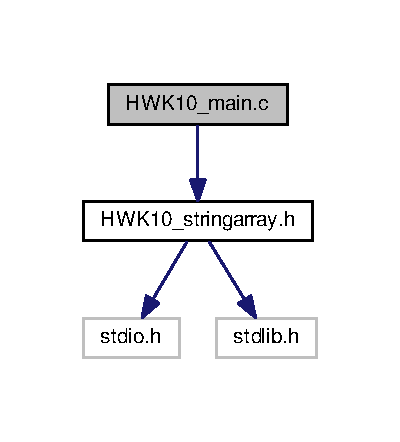
\includegraphics[width=192pt]{HWK10__main_8c__incl}
\end{center}
\end{figure}
\subsection*{Macros}
\begin{DoxyCompactItemize}
\item 
\#define \hyperlink{HWK10__main_8c_a78d344caabde729a4559393a0552bf1c}{A\+R\+R\+A\+Y\+S\+I\+ZE}~2000
\end{DoxyCompactItemize}
\subsection*{Functions}
\begin{DoxyCompactItemize}
\item 
int \hyperlink{HWK10__main_8c_a840291bc02cba5474a4cb46a9b9566fe}{main} (void)
\end{DoxyCompactItemize}


\subsection{Macro Definition Documentation}
\index{H\+W\+K10\+\_\+main.\+c@{H\+W\+K10\+\_\+main.\+c}!A\+R\+R\+A\+Y\+S\+I\+ZE@{A\+R\+R\+A\+Y\+S\+I\+ZE}}
\index{A\+R\+R\+A\+Y\+S\+I\+ZE@{A\+R\+R\+A\+Y\+S\+I\+ZE}!H\+W\+K10\+\_\+main.\+c@{H\+W\+K10\+\_\+main.\+c}}
\subsubsection[{\texorpdfstring{A\+R\+R\+A\+Y\+S\+I\+ZE}{ARRAYSIZE}}]{\setlength{\rightskip}{0pt plus 5cm}\#define A\+R\+R\+A\+Y\+S\+I\+ZE~2000}\hypertarget{HWK10__main_8c_a78d344caabde729a4559393a0552bf1c}{}\label{HWK10__main_8c_a78d344caabde729a4559393a0552bf1c}


\subsection{Function Documentation}
\index{H\+W\+K10\+\_\+main.\+c@{H\+W\+K10\+\_\+main.\+c}!main@{main}}
\index{main@{main}!H\+W\+K10\+\_\+main.\+c@{H\+W\+K10\+\_\+main.\+c}}
\subsubsection[{\texorpdfstring{main(void)}{main(void)}}]{\setlength{\rightskip}{0pt plus 5cm}int main (
\begin{DoxyParamCaption}
\item[{void}]{}
\end{DoxyParamCaption}
)}\hypertarget{HWK10__main_8c_a840291bc02cba5474a4cb46a9b9566fe}{}\label{HWK10__main_8c_a840291bc02cba5474a4cb46a9b9566fe}

\begin{DoxyCode}
10               \{
11   \textcolor{keywordtype}{int} n;
12   \hyperlink{HWK10__stringarray_8h_a9e38333c54335607829268149cf3855a}{linetype} linearray[\hyperlink{HWK10__main_8c_a78d344caabde729a4559393a0552bf1c}{ARRAYSIZE}];
13   \hyperlink{HWK10__stringarray_8h_a9e38333c54335607829268149cf3855a}{linetype} who;
14   \textcolor{keywordtype}{int} where;
15   FILE *fdw;  \textcolor{comment}{/* FILE descriptor used for "who.dat" */}
16   FILE *fda;  \textcolor{comment}{/* File descriptor used for "answers.dat" */}
17   
18   \textcolor{comment}{/* Read unsorted.dat into linearray and return number of lines read */}
19   n = \hyperlink{HWK10__stringarray_8c_ae87b96e9c69a38ef44d8915a2a76a2d6}{getStringArray}(\textcolor{stringliteral}{"unsorted.dat"}, linearray, \hyperlink{HWK10__main_8c_a78d344caabde729a4559393a0552bf1c}{ARRAYSIZE});
20   \textcolor{keywordflow}{if} (n==0)\{
21     printf(\textcolor{stringliteral}{"The unsorted.dat file is empty. Good bye.\(\backslash\)n"});
22     exit(0);
23   \}
24   \textcolor{comment}{/* Sort the first n lines of linearray */}
25   \hyperlink{HWK10__stringarray_8c_ac29b7bb6177ffab2b99341426b422b03}{stringBubble}(linearray,n);
26   \textcolor{comment}{/* Save the sorted array to sorted.dat */}
27   \hyperlink{HWK10__stringarray_8c_a15bea2142e99a70219bb49e6ff400f9d}{writeStringArray}(\textcolor{stringliteral}{"sorted.dat"},linearray,n);
28   \textcolor{comment}{/* Open for reading who.dat */}
29   \textcolor{keywordflow}{if}((fdw=fopen(\textcolor{stringliteral}{"who.dat"},\textcolor{stringliteral}{"r"}))==NULL)\{
30     perror(\textcolor{stringliteral}{"fopen"});
31     exit(1);
32   \}
33   \textcolor{comment}{/* Open for writing answers.dat */}
34   \textcolor{keywordflow}{if}((fda=fopen(\textcolor{stringliteral}{"answers.dat"},\textcolor{stringliteral}{"w"}))==NULL)\{
35     perror(\textcolor{stringliteral}{"fopen"});
36     exit(1);
37   \}
38   \textcolor{keywordflow}{while} (\hyperlink{HWK10__stringarray_8c_afe9546ca2b716582998ebfac1ca6ff99}{getlineX}(fdw,who,\hyperlink{HWK10__stringarray_8h_a0095c1e0ae26941efea12c77f2232f2f}{LINESIZE}-1)!=EOF)\{   \textcolor{comment}{/* Read a line from "who.dat" */}
39     where = \hyperlink{HWK10__stringarray_8c_a594e6934fc18035c2a074fa079a50515}{stringBinary}(linearray,n,who);    \textcolor{comment}{/* See where it is in table */}
40     fprintf(fda,\textcolor{stringliteral}{"%d\(\backslash\)n"},where);            \textcolor{comment}{/* Write position to "answer.dat*/}
41   \}
42   fclose(fdw);
43   fclose(fda);
44 \}
\end{DoxyCode}


Here is the call graph for this function\+:
\nopagebreak
\begin{figure}[H]
\begin{center}
\leavevmode
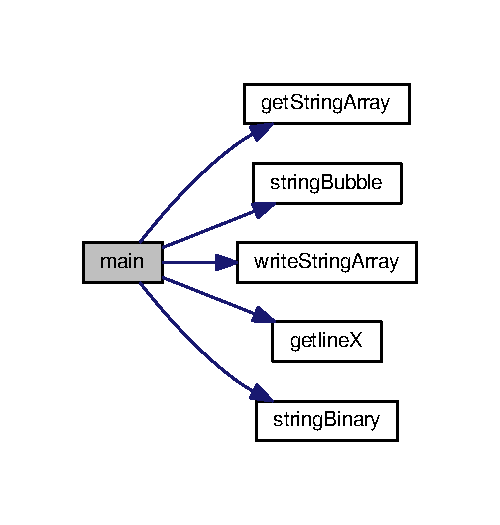
\includegraphics[width=240pt]{HWK10__main_8c_a840291bc02cba5474a4cb46a9b9566fe_cgraph}
\end{center}
\end{figure}



\hypertarget{HWK10__stringarray_8c}{}\section{H\+W\+K10\+\_\+stringarray.\+c File Reference}
\label{HWK10__stringarray_8c}\index{H\+W\+K10\+\_\+stringarray.\+c@{H\+W\+K10\+\_\+stringarray.\+c}}
{\ttfamily \#include \char`\"{}H\+W\+K10\+\_\+stringarray.\+h\char`\"{}}\\*
Include dependency graph for H\+W\+K10\+\_\+stringarray.\+c\+:
\nopagebreak
\begin{figure}[H]
\begin{center}
\leavevmode
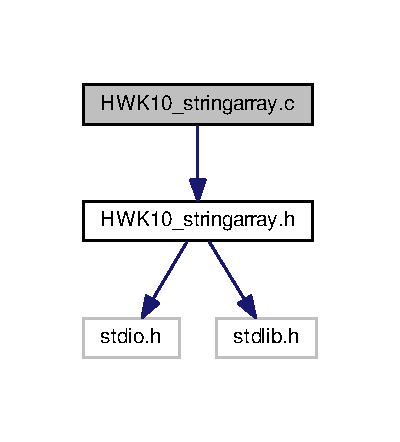
\includegraphics[width=192pt]{HWK10__stringarray_8c__incl}
\end{center}
\end{figure}
\subsection*{Functions}
\begin{DoxyCompactItemize}
\item 
int \hyperlink{HWK10__stringarray_8c_afe9546ca2b716582998ebfac1ca6ff99}{getlineX} (F\+I\+LE $\ast$fd, char buff\mbox{[}$\,$\mbox{]}, int nmax)
\item 
int \hyperlink{HWK10__stringarray_8c_ae87b96e9c69a38ef44d8915a2a76a2d6}{get\+String\+Array} (char $\ast$filename, \hyperlink{HWK10__stringarray_8h_a9e38333c54335607829268149cf3855a}{linetype} table\mbox{[}$\,$\mbox{]}, int nmax)
\item 
void \hyperlink{HWK10__stringarray_8c_a15bea2142e99a70219bb49e6ff400f9d}{write\+String\+Array} (char $\ast$filename, \hyperlink{HWK10__stringarray_8h_a9e38333c54335607829268149cf3855a}{linetype} table\mbox{[}$\,$\mbox{]}, int n)
\item 
void \hyperlink{HWK10__stringarray_8c_ac29b7bb6177ffab2b99341426b422b03}{string\+Bubble} (\hyperlink{HWK10__stringarray_8h_a9e38333c54335607829268149cf3855a}{linetype} table\mbox{[}$\,$\mbox{]}, int n)
\item 
int \hyperlink{HWK10__stringarray_8c_a594e6934fc18035c2a074fa079a50515}{string\+Binary} (\hyperlink{HWK10__stringarray_8h_a9e38333c54335607829268149cf3855a}{linetype} table\mbox{[}$\,$\mbox{]}, int n, char who\mbox{[}$\,$\mbox{]})
\end{DoxyCompactItemize}


\subsection{Function Documentation}
\index{H\+W\+K10\+\_\+stringarray.\+c@{H\+W\+K10\+\_\+stringarray.\+c}!getlineX@{getlineX}}
\index{getlineX@{getlineX}!H\+W\+K10\+\_\+stringarray.\+c@{H\+W\+K10\+\_\+stringarray.\+c}}
\subsubsection[{\texorpdfstring{getline\+X(\+F\+I\+L\+E $\ast$fd, char buff[], int nmax)}{getlineX(FILE *fd, char buff[], int nmax)}}]{\setlength{\rightskip}{0pt plus 5cm}int getlineX (
\begin{DoxyParamCaption}
\item[{F\+I\+LE $\ast$}]{fd, }
\item[{char}]{buff\mbox{[}$\,$\mbox{]}, }
\item[{int}]{nmax}
\end{DoxyParamCaption}
)}\hypertarget{HWK10__stringarray_8c_afe9546ca2b716582998ebfac1ca6ff99}{}\label{HWK10__stringarray_8c_afe9546ca2b716582998ebfac1ca6ff99}

\begin{DoxyCode}
6                                               \{
7   \textcolor{comment}{/* It reads a line from fd and stores up to nmax of 
}
8 \textcolor{comment}{   * its characters to buff.
}
9 \textcolor{comment}{   */}
10   \textcolor{keywordtype}{char} c;
11   \textcolor{keywordtype}{int} n=0;
12 
13   \textcolor{keywordflow}{while} ((c=getc(fd))!=\textcolor{charliteral}{'\(\backslash\)n'})\{
14     \textcolor{keywordflow}{if}(c==EOF)\textcolor{keywordflow}{return} EOF;
15     \textcolor{keywordflow}{if}(n<nmax)
16       buff[n++]=c;
17   \}
18   buff[n]=\textcolor{charliteral}{'\(\backslash\)0'};
19   \textcolor{keywordflow}{return} n;
20 \}
\end{DoxyCode}
\index{H\+W\+K10\+\_\+stringarray.\+c@{H\+W\+K10\+\_\+stringarray.\+c}!get\+String\+Array@{get\+String\+Array}}
\index{get\+String\+Array@{get\+String\+Array}!H\+W\+K10\+\_\+stringarray.\+c@{H\+W\+K10\+\_\+stringarray.\+c}}
\subsubsection[{\texorpdfstring{get\+String\+Array(char $\ast$filename, linetype table[], int nmax)}{getStringArray(char *filename, linetype table[], int nmax)}}]{\setlength{\rightskip}{0pt plus 5cm}int get\+String\+Array (
\begin{DoxyParamCaption}
\item[{char $\ast$}]{filename, }
\item[{{\bf linetype}}]{table\mbox{[}$\,$\mbox{]}, }
\item[{int}]{nmax}
\end{DoxyParamCaption}
)}\hypertarget{HWK10__stringarray_8c_ae87b96e9c69a38ef44d8915a2a76a2d6}{}\label{HWK10__stringarray_8c_ae87b96e9c69a38ef44d8915a2a76a2d6}

\begin{DoxyCode}
26 \{
27   FILE *fdu;  \textcolor{comment}{/* File descriptor used for filename */}
28   \textcolor{keywordtype}{int} i, j;
29   \textcolor{keywordtype}{char} c;
30 
31   \textcolor{keywordflow}{if}((fdu=fopen(filename,\textcolor{stringliteral}{"r"}))==NULL)\{
32     perror(\textcolor{stringliteral}{"fopen"});
33     exit(1);
34   \}
35   i=j=0;
36   \textcolor{keywordflow}{while}((c=getc(fdu))!=EOF)\{
37     \textcolor{keywordflow}{if}(i==nmax)\textcolor{keywordflow}{break};  \textcolor{comment}{/* We have filled up the table */}
38     \textcolor{keywordflow}{if} (c==\textcolor{charliteral}{'\(\backslash\)n'})\{ \textcolor{comment}{/* We have finished reading a line */}
39       table[i++][j]=\textcolor{charliteral}{'\(\backslash\)0'};
40       j=0;
41     \}\textcolor{keywordflow}{else} \textcolor{keywordflow}{if}(j<\hyperlink{HWK10__stringarray_8h_a0095c1e0ae26941efea12c77f2232f2f}{LINESIZE})
42       table[i][j++]=c;
43   \}
44   fclose(fdu);
45   \textcolor{keywordflow}{return} i;
46 \}
\end{DoxyCode}
\index{H\+W\+K10\+\_\+stringarray.\+c@{H\+W\+K10\+\_\+stringarray.\+c}!string\+Binary@{string\+Binary}}
\index{string\+Binary@{string\+Binary}!H\+W\+K10\+\_\+stringarray.\+c@{H\+W\+K10\+\_\+stringarray.\+c}}
\subsubsection[{\texorpdfstring{string\+Binary(linetype table[], int n, char who[])}{stringBinary(linetype table[], int n, char who[])}}]{\setlength{\rightskip}{0pt plus 5cm}int string\+Binary (
\begin{DoxyParamCaption}
\item[{{\bf linetype}}]{table\mbox{[}$\,$\mbox{]}, }
\item[{int}]{n, }
\item[{char}]{who\mbox{[}$\,$\mbox{]}}
\end{DoxyParamCaption}
)}\hypertarget{HWK10__stringarray_8c_a594e6934fc18035c2a074fa079a50515}{}\label{HWK10__stringarray_8c_a594e6934fc18035c2a074fa079a50515}

\begin{DoxyCode}
71                                                      \{
72   \textcolor{comment}{/* It searches the first n positions of table looking for who.
}
73 \textcolor{comment}{   * It uses binary search. It returns the position where who is
}
74 \textcolor{comment}{   * found, or -1 if not there. This is just the prototype, or stub, 
}
75 \textcolor{comment}{   * of the function.
}
76 \textcolor{comment}{   */}
77   \textcolor{keywordflow}{return} -1;
78 \}
\end{DoxyCode}
\index{H\+W\+K10\+\_\+stringarray.\+c@{H\+W\+K10\+\_\+stringarray.\+c}!string\+Bubble@{string\+Bubble}}
\index{string\+Bubble@{string\+Bubble}!H\+W\+K10\+\_\+stringarray.\+c@{H\+W\+K10\+\_\+stringarray.\+c}}
\subsubsection[{\texorpdfstring{string\+Bubble(linetype table[], int n)}{stringBubble(linetype table[], int n)}}]{\setlength{\rightskip}{0pt plus 5cm}void string\+Bubble (
\begin{DoxyParamCaption}
\item[{{\bf linetype}}]{table\mbox{[}$\,$\mbox{]}, }
\item[{int}]{n}
\end{DoxyParamCaption}
)}\hypertarget{HWK10__stringarray_8c_ac29b7bb6177ffab2b99341426b422b03}{}\label{HWK10__stringarray_8c_ac29b7bb6177ffab2b99341426b422b03}

\begin{DoxyCode}
65                                           \{
66   \textcolor{comment}{/* This function sorts the first n lines of table.
}
67 \textcolor{comment}{   * Here you see just the prototype, or stub, of the function.
}
68 \textcolor{comment}{   */}
69 \}
\end{DoxyCode}
\index{H\+W\+K10\+\_\+stringarray.\+c@{H\+W\+K10\+\_\+stringarray.\+c}!write\+String\+Array@{write\+String\+Array}}
\index{write\+String\+Array@{write\+String\+Array}!H\+W\+K10\+\_\+stringarray.\+c@{H\+W\+K10\+\_\+stringarray.\+c}}
\subsubsection[{\texorpdfstring{write\+String\+Array(char $\ast$filename, linetype table[], int n)}{writeStringArray(char *filename, linetype table[], int n)}}]{\setlength{\rightskip}{0pt plus 5cm}void write\+String\+Array (
\begin{DoxyParamCaption}
\item[{char $\ast$}]{filename, }
\item[{{\bf linetype}}]{table\mbox{[}$\,$\mbox{]}, }
\item[{int}]{n}
\end{DoxyParamCaption}
)}\hypertarget{HWK10__stringarray_8c_a15bea2142e99a70219bb49e6ff400f9d}{}\label{HWK10__stringarray_8c_a15bea2142e99a70219bb49e6ff400f9d}

\begin{DoxyCode}
52 \{
53   FILE *fdu;  \textcolor{comment}{/* File descriptor used for filename */}
54   \textcolor{keywordtype}{int} i;
55   
56   \textcolor{keywordflow}{if}((fdu=fopen(filename,\textcolor{stringliteral}{"w"}))==NULL)\{
57     perror(\textcolor{stringliteral}{"fopen"});
58     exit(1);
59   \}
60   \textcolor{keywordflow}{for}(i=0;i<n;i++)
61     fprintf(fdu, \textcolor{stringliteral}{"%s\(\backslash\)n"}, table[i]);
62   fclose(fdu);
63 \}
\end{DoxyCode}

\hypertarget{HWK10__stringarray_8h}{}\section{H\+W\+K10\+\_\+stringarray.\+h File Reference}
\label{HWK10__stringarray_8h}\index{H\+W\+K10\+\_\+stringarray.\+h@{H\+W\+K10\+\_\+stringarray.\+h}}
{\ttfamily \#include $<$stdio.\+h$>$}\\*
{\ttfamily \#include $<$stdlib.\+h$>$}\\*
Include dependency graph for H\+W\+K10\+\_\+stringarray.\+h\+:
\nopagebreak
\begin{figure}[H]
\begin{center}
\leavevmode
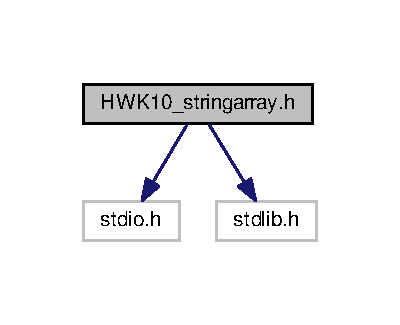
\includegraphics[width=192pt]{HWK10__stringarray_8h__incl}
\end{center}
\end{figure}
This graph shows which files directly or indirectly include this file\+:
\nopagebreak
\begin{figure}[H]
\begin{center}
\leavevmode
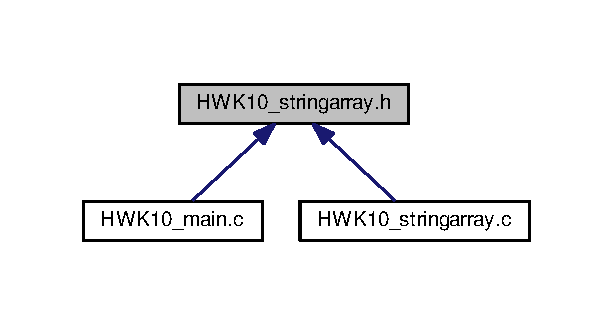
\includegraphics[width=294pt]{HWK10__stringarray_8h__dep__incl}
\end{center}
\end{figure}
\subsection*{Macros}
\begin{DoxyCompactItemize}
\item 
\#define \hyperlink{HWK10__stringarray_8h_a0095c1e0ae26941efea12c77f2232f2f}{L\+I\+N\+E\+S\+I\+ZE}~65
\end{DoxyCompactItemize}
\subsection*{Typedefs}
\begin{DoxyCompactItemize}
\item 
typedef char \hyperlink{HWK10__stringarray_8h_a9e38333c54335607829268149cf3855a}{linetype}\mbox{[}\hyperlink{HWK10__stringarray_8h_a0095c1e0ae26941efea12c77f2232f2f}{L\+I\+N\+E\+S\+I\+ZE}\mbox{]}
\end{DoxyCompactItemize}
\subsection*{Functions}
\begin{DoxyCompactItemize}
\item 
int \hyperlink{HWK10__stringarray_8h_afe9546ca2b716582998ebfac1ca6ff99}{getlineX} (F\+I\+LE $\ast$fd, char buff\mbox{[}$\,$\mbox{]}, int nmax)
\item 
int \hyperlink{HWK10__stringarray_8h_ae87b96e9c69a38ef44d8915a2a76a2d6}{get\+String\+Array} (char $\ast$filename, \hyperlink{HWK10__stringarray_8h_a9e38333c54335607829268149cf3855a}{linetype} table\mbox{[}$\,$\mbox{]}, int nmax)
\item 
void \hyperlink{HWK10__stringarray_8h_a15bea2142e99a70219bb49e6ff400f9d}{write\+String\+Array} (char $\ast$filename, \hyperlink{HWK10__stringarray_8h_a9e38333c54335607829268149cf3855a}{linetype} table\mbox{[}$\,$\mbox{]}, int n)
\item 
void \hyperlink{HWK10__stringarray_8h_ac29b7bb6177ffab2b99341426b422b03}{string\+Bubble} (\hyperlink{HWK10__stringarray_8h_a9e38333c54335607829268149cf3855a}{linetype} table\mbox{[}$\,$\mbox{]}, int n)
\item 
int \hyperlink{HWK10__stringarray_8h_a594e6934fc18035c2a074fa079a50515}{string\+Binary} (\hyperlink{HWK10__stringarray_8h_a9e38333c54335607829268149cf3855a}{linetype} table\mbox{[}$\,$\mbox{]}, int n, char who\mbox{[}$\,$\mbox{]})
\end{DoxyCompactItemize}


\subsection{Macro Definition Documentation}
\index{H\+W\+K10\+\_\+stringarray.\+h@{H\+W\+K10\+\_\+stringarray.\+h}!L\+I\+N\+E\+S\+I\+ZE@{L\+I\+N\+E\+S\+I\+ZE}}
\index{L\+I\+N\+E\+S\+I\+ZE@{L\+I\+N\+E\+S\+I\+ZE}!H\+W\+K10\+\_\+stringarray.\+h@{H\+W\+K10\+\_\+stringarray.\+h}}
\subsubsection[{\texorpdfstring{L\+I\+N\+E\+S\+I\+ZE}{LINESIZE}}]{\setlength{\rightskip}{0pt plus 5cm}\#define L\+I\+N\+E\+S\+I\+ZE~65}\hypertarget{HWK10__stringarray_8h_a0095c1e0ae26941efea12c77f2232f2f}{}\label{HWK10__stringarray_8h_a0095c1e0ae26941efea12c77f2232f2f}


\subsection{Typedef Documentation}
\index{H\+W\+K10\+\_\+stringarray.\+h@{H\+W\+K10\+\_\+stringarray.\+h}!linetype@{linetype}}
\index{linetype@{linetype}!H\+W\+K10\+\_\+stringarray.\+h@{H\+W\+K10\+\_\+stringarray.\+h}}
\subsubsection[{\texorpdfstring{linetype}{linetype}}]{\setlength{\rightskip}{0pt plus 5cm}typedef char linetype\mbox{[}{\bf L\+I\+N\+E\+S\+I\+ZE}\mbox{]}}\hypertarget{HWK10__stringarray_8h_a9e38333c54335607829268149cf3855a}{}\label{HWK10__stringarray_8h_a9e38333c54335607829268149cf3855a}


\subsection{Function Documentation}
\index{H\+W\+K10\+\_\+stringarray.\+h@{H\+W\+K10\+\_\+stringarray.\+h}!getlineX@{getlineX}}
\index{getlineX@{getlineX}!H\+W\+K10\+\_\+stringarray.\+h@{H\+W\+K10\+\_\+stringarray.\+h}}
\subsubsection[{\texorpdfstring{getline\+X(\+F\+I\+L\+E $\ast$fd, char buff[], int nmax)}{getlineX(FILE *fd, char buff[], int nmax)}}]{\setlength{\rightskip}{0pt plus 5cm}int getlineX (
\begin{DoxyParamCaption}
\item[{F\+I\+LE $\ast$}]{fd, }
\item[{char}]{buff\mbox{[}$\,$\mbox{]}, }
\item[{int}]{nmax}
\end{DoxyParamCaption}
)}\hypertarget{HWK10__stringarray_8h_afe9546ca2b716582998ebfac1ca6ff99}{}\label{HWK10__stringarray_8h_afe9546ca2b716582998ebfac1ca6ff99}

\begin{DoxyCode}
6                                               \{
7   \textcolor{comment}{/* It reads a line from fd and stores up to nmax of 
}
8 \textcolor{comment}{   * its characters to buff.
}
9 \textcolor{comment}{   */}
10   \textcolor{keywordtype}{char} c;
11   \textcolor{keywordtype}{int} n=0;
12 
13   \textcolor{keywordflow}{while} ((c=getc(fd))!=\textcolor{charliteral}{'\(\backslash\)n'})\{
14     \textcolor{keywordflow}{if}(c==EOF)\textcolor{keywordflow}{return} EOF;
15     \textcolor{keywordflow}{if}(n<nmax)
16       buff[n++]=c;
17   \}
18   buff[n]=\textcolor{charliteral}{'\(\backslash\)0'};
19   \textcolor{keywordflow}{return} n;
20 \}
\end{DoxyCode}
\index{H\+W\+K10\+\_\+stringarray.\+h@{H\+W\+K10\+\_\+stringarray.\+h}!get\+String\+Array@{get\+String\+Array}}
\index{get\+String\+Array@{get\+String\+Array}!H\+W\+K10\+\_\+stringarray.\+h@{H\+W\+K10\+\_\+stringarray.\+h}}
\subsubsection[{\texorpdfstring{get\+String\+Array(char $\ast$filename, linetype table[], int nmax)}{getStringArray(char *filename, linetype table[], int nmax)}}]{\setlength{\rightskip}{0pt plus 5cm}int get\+String\+Array (
\begin{DoxyParamCaption}
\item[{char $\ast$}]{filename, }
\item[{{\bf linetype}}]{table\mbox{[}$\,$\mbox{]}, }
\item[{int}]{nmax}
\end{DoxyParamCaption}
)}\hypertarget{HWK10__stringarray_8h_ae87b96e9c69a38ef44d8915a2a76a2d6}{}\label{HWK10__stringarray_8h_ae87b96e9c69a38ef44d8915a2a76a2d6}

\begin{DoxyCode}
26 \{
27   FILE *fdu;  \textcolor{comment}{/* File descriptor used for filename */}
28   \textcolor{keywordtype}{int} i, j;
29   \textcolor{keywordtype}{char} c;
30 
31   \textcolor{keywordflow}{if}((fdu=fopen(filename,\textcolor{stringliteral}{"r"}))==NULL)\{
32     perror(\textcolor{stringliteral}{"fopen"});
33     exit(1);
34   \}
35   i=j=0;
36   \textcolor{keywordflow}{while}((c=getc(fdu))!=EOF)\{
37     \textcolor{keywordflow}{if}(i==nmax)\textcolor{keywordflow}{break};  \textcolor{comment}{/* We have filled up the table */}
38     \textcolor{keywordflow}{if} (c==\textcolor{charliteral}{'\(\backslash\)n'})\{ \textcolor{comment}{/* We have finished reading a line */}
39       table[i++][j]=\textcolor{charliteral}{'\(\backslash\)0'};
40       j=0;
41     \}\textcolor{keywordflow}{else} \textcolor{keywordflow}{if}(j<\hyperlink{HWK10__stringarray_8h_a0095c1e0ae26941efea12c77f2232f2f}{LINESIZE})
42       table[i][j++]=c;
43   \}
44   fclose(fdu);
45   \textcolor{keywordflow}{return} i;
46 \}
\end{DoxyCode}
\index{H\+W\+K10\+\_\+stringarray.\+h@{H\+W\+K10\+\_\+stringarray.\+h}!string\+Binary@{string\+Binary}}
\index{string\+Binary@{string\+Binary}!H\+W\+K10\+\_\+stringarray.\+h@{H\+W\+K10\+\_\+stringarray.\+h}}
\subsubsection[{\texorpdfstring{string\+Binary(linetype table[], int n, char who[])}{stringBinary(linetype table[], int n, char who[])}}]{\setlength{\rightskip}{0pt plus 5cm}int string\+Binary (
\begin{DoxyParamCaption}
\item[{{\bf linetype}}]{table\mbox{[}$\,$\mbox{]}, }
\item[{int}]{n, }
\item[{char}]{who\mbox{[}$\,$\mbox{]}}
\end{DoxyParamCaption}
)}\hypertarget{HWK10__stringarray_8h_a594e6934fc18035c2a074fa079a50515}{}\label{HWK10__stringarray_8h_a594e6934fc18035c2a074fa079a50515}

\begin{DoxyCode}
71                                                      \{
72   \textcolor{comment}{/* It searches the first n positions of table looking for who.
}
73 \textcolor{comment}{   * It uses binary search. It returns the position where who is
}
74 \textcolor{comment}{   * found, or -1 if not there. This is just the prototype, or stub, 
}
75 \textcolor{comment}{   * of the function.
}
76 \textcolor{comment}{   */}
77   \textcolor{keywordflow}{return} -1;
78 \}
\end{DoxyCode}
\index{H\+W\+K10\+\_\+stringarray.\+h@{H\+W\+K10\+\_\+stringarray.\+h}!string\+Bubble@{string\+Bubble}}
\index{string\+Bubble@{string\+Bubble}!H\+W\+K10\+\_\+stringarray.\+h@{H\+W\+K10\+\_\+stringarray.\+h}}
\subsubsection[{\texorpdfstring{string\+Bubble(linetype table[], int n)}{stringBubble(linetype table[], int n)}}]{\setlength{\rightskip}{0pt plus 5cm}void string\+Bubble (
\begin{DoxyParamCaption}
\item[{{\bf linetype}}]{table\mbox{[}$\,$\mbox{]}, }
\item[{int}]{n}
\end{DoxyParamCaption}
)}\hypertarget{HWK10__stringarray_8h_ac29b7bb6177ffab2b99341426b422b03}{}\label{HWK10__stringarray_8h_ac29b7bb6177ffab2b99341426b422b03}

\begin{DoxyCode}
65                                           \{
66   \textcolor{comment}{/* This function sorts the first n lines of table.
}
67 \textcolor{comment}{   * Here you see just the prototype, or stub, of the function.
}
68 \textcolor{comment}{   */}
69 \}
\end{DoxyCode}
\index{H\+W\+K10\+\_\+stringarray.\+h@{H\+W\+K10\+\_\+stringarray.\+h}!write\+String\+Array@{write\+String\+Array}}
\index{write\+String\+Array@{write\+String\+Array}!H\+W\+K10\+\_\+stringarray.\+h@{H\+W\+K10\+\_\+stringarray.\+h}}
\subsubsection[{\texorpdfstring{write\+String\+Array(char $\ast$filename, linetype table[], int n)}{writeStringArray(char *filename, linetype table[], int n)}}]{\setlength{\rightskip}{0pt plus 5cm}void write\+String\+Array (
\begin{DoxyParamCaption}
\item[{char $\ast$}]{filename, }
\item[{{\bf linetype}}]{table\mbox{[}$\,$\mbox{]}, }
\item[{int}]{n}
\end{DoxyParamCaption}
)}\hypertarget{HWK10__stringarray_8h_a15bea2142e99a70219bb49e6ff400f9d}{}\label{HWK10__stringarray_8h_a15bea2142e99a70219bb49e6ff400f9d}

\begin{DoxyCode}
52 \{
53   FILE *fdu;  \textcolor{comment}{/* File descriptor used for filename */}
54   \textcolor{keywordtype}{int} i;
55   
56   \textcolor{keywordflow}{if}((fdu=fopen(filename,\textcolor{stringliteral}{"w"}))==NULL)\{
57     perror(\textcolor{stringliteral}{"fopen"});
58     exit(1);
59   \}
60   \textcolor{keywordflow}{for}(i=0;i<n;i++)
61     fprintf(fdu, \textcolor{stringliteral}{"%s\(\backslash\)n"}, table[i]);
62   fclose(fdu);
63 \}
\end{DoxyCode}

%--- End generated contents ---

% Index
\backmatter
\newpage
\phantomsection
\clearemptydoublepage
\addcontentsline{toc}{chapter}{Index}
\printindex

\end{document}
